\documentclass{beamer}
\usetheme{Madrid}
\usecolortheme{default}
\usepackage{comment}
\usepackage[table,xcdraw]{xcolor}
\usepackage{booktabs}
\usepackage{pgfplots}
\title[Mid-Term Presentation]
{Multi-class link prediction with PyKEEN and Large Language Models}



\author[] % (optional, for multiple authors)
{William Liaw \and Sriraam Appakutti Palani  \and Eddie Groh\and \\Mochamad Ardiansyah Nurgaha}

\institute[Team: AWESome] % (optional)
{%
  Mehwish ALAM\\
  Associate Professor
  \and
  Language Models and Structured Data\\
}

\date[9 January 2025] % (optional)
{9 January 2025}

\logo{}

\definecolor{uoftblue}{RGB}{6,41,88}
\setbeamercolor{titlelike}{bg=uoftblue}
\setbeamerfont{title}{series=\bfseries}

\begin{document}

\frame{\titlepage}
\begin{frame}
    \frametitle{Table of Contents}
    \tableofcontents
\end{frame}

\section{Introduction}
\begin{frame}
    \begin{columns}
        \frametitle{Introduction}

        % Left Column
        \column{0.5\textwidth}
        \begin{minipage}{\dimexpr\textwidth-2\fboxsep}
            \begin{center}
                \textbf{Knowledge Graph Completion} \\[1em]
            \end{center}
            \small \textbf{Goal:} Predict missing links to complete and enhance knowledge graphs. \\[0.5em]
            \small \textbf{Methods:} Use embedding models, LLM-based techniques, and hybrid approaches.
        \end{minipage}

        % Right Column
        \column{0.5\textwidth}
        \colorbox{blue!10}{
            \begin{minipage}{\dimexpr\textwidth-2\fboxsep}
                \begin{center}
                    \includegraphics[width=0.3\textwidth]{images/pykeen-logo} \\
                    \textbf{Py}thon \textbf{K}nowledge \textbf{E}mbedding and \textbf{E}valuation \textbf{N}etwork \\[1em]
                \end{center}
                \small \textbf{Purpose:} Knowledge graph embedding and link prediction tasks. \\[1.2em]

                \begin{center}
                    \includegraphics[width=0.3\textwidth]{images/neo4j-logo} \\
                    \textbf{Neo4j Desktop} \\[1em]
                \end{center}
                \small \textbf{Purpose:} Neo4j is a graph database designed to store and manage connected data.
            \end{minipage}
        }
    \end{columns}
\end{frame}

\begin{frame}
    \frametitle{Goal \& Motivation}
    \centering
    How to predict missing links to complete and enhance knowledge graphs with LLMs? \\[2em]
    \includegraphics[width=0.7\textwidth]{images/motivation} \\
\end{frame}

\begin{frame}{Problem Statement}
    \textbf{\textit{Motivation:}} Knowledge graphs are often incomplete, limiting applications like
    \begin{itemize}
        \item Recommendation systems
        \item Biomedical research
        \item Drug repurposing
    \end{itemize}
    \textbf{\textit{Objective:}} Address incompleteness by
    \begin{enumerate}
        \item Employing PyKEEN for link prediction and relationship classification.
        \item Exploring LLMs to complement traditional methods.
    \end{enumerate}
\end{frame}





\section{Methodology}
\begin{frame}{Methodology Overview}
    \begin{enumerate}
        \item PyKEEN: \\
              \begin{itemize}
                  \item Enables KGE models over entities and relations into vector spaces.
                  \item Facilitates link prediction and multi-class classification.
              \end{itemize}
        \item Neo4j:
              \begin{itemize}
                  \item Query and manage the graph data.
                  \item Retrieve triples (h, r, t) for PyKEEN training.
              \end{itemize}
        \item LLM Integration:
              \begin{itemize}
                  \item Dual embedding architecture of RotatE with LLaMA 3.2-3B
                  \item Future exploration on zero-shot, few-shot, and RAG techniques.
              \end{itemize}
    \end{enumerate}
\end{frame}





\begin{frame}{PyKEEN Setup}
    \begin{block}{Extract triples using Cypher query}
        \scriptsize MATCH (h)-[r] $\rightarrow$ (t) \\
        RETURN id(h) AS head, type(r) AS relation, id(t) AS tail
    \end{block}

    \begin{block}{Convert triples to PyKEEN’s TriplesFactory format}
        \scriptsize For example: [("Gene\_A", "causes", "Disease\_X")] $\rightarrow$ [0, 0, 1] \\
        \begin{itemize}
            \item These ID mappings are used during model training.
        \end{itemize}
    \end{block}

    \begin{block}{Train using RotatE model with}
        \begin{itemize}
            \item \small 100 epochs
            \item \small Embedding dimension = 128
            \item \small Family of KGE models tested.
        \end{itemize}
    \end{block}
\end{frame}




\begin{frame}{Neo4j and LLMs Integration}

    \begin{block}{Neo4j Integration}
        \begin{itemize}
            \item \small Setup Neo4j Desktop with Hetionet Database.
            \item \small Visualize Schema using \tiny CALL db.schema.visualization().
        \end{itemize}
    \end{block}

    \begin{block}{LLMs (Dual Embedding Architecture)}
        \small \textbf{\textit{Integrating RotatE with LLaMA 3.2-3B for Knowledge Graph Embeddings\\}}
        \textbf{\textit{\small \\Key Components:}}

        \begin{itemize}
            \item \textbf{\textit{\small RotatE:}} Traditional entity and relation embeddings in complex space, trained using PyKEEN.
            \item \textbf{\textit{\small LLaMA 3.2-3B (RLM-A):}} LLM embeddings, initialized with Wikidata entries for entities.
        \end{itemize}
        \textbf{\textit{This semantic-rich embeddings enhances link prediction.}}

    \end{block}

\end{frame}


\section{Experimental Setup and Key Metrics}

\begin{frame}{Experimental Setup}

    \textbf{Hetionet:}

    \begin{minipage}{0.49\textwidth}
        \begin{itemize}
            \item \small Biomedical knowledge graph representing relationships between diseases, drugs, genes, and other biological entities.
            \item \small High edge-to-node ratio
        \end{itemize}
    \end{minipage}
    \hfill
    \begin{minipage}{0.50\textwidth}
        \begin{table}
            \small
            \rowcolors{2}{gray!15}{white}
            \begin{tabular}{l c}
                \toprule
                \textbf{Statistic}    & \textbf{Value} \\ \midrule
                Entities (Nodes )     & 22,634         \\
                Relationships (Edges) & 561,721        \\
                Unique Relation Types & 10             \\
                Unique Triples        & 561,721        \\ \bottomrule
            \end{tabular}
        \end{table}
        \hfill
    \end{minipage}

    \textbf{Evaluation Metrics:}

    \begin{itemize}
        \item \small Hits@K - Fraction of correct predictions ranked in the top K.
        \item \small Mean Reciprocal Rank (MRR) -  Average inverse rank of correct predictions.
        \item \small Mean Rank (MR) - Average rank of correct predictions.
    \end{itemize}

\end{frame}

\begin{frame}{Model Comparison}
    \begin{tikzpicture}
        \begin{axis}[
                ybar,
                width=\textwidth,
                height=0.8\textheight,
                yticklabel style={/pgf/number format/fixed},
                symbolic x coords={Hits@1, Hits@3, Hits@5, Hits@10, MRR, MRt},
                legend style={at={(0.5,-0.15)}, anchor=north, legend columns=-1},
                legend cell align={left},
                grid=major,
                enlarge x limits=0.15,
            ]
            % Add data for RLM-A
            \addplot coordinates {(Hits@1, 0.0260) (Hits@3, 0.0564) (Hits@5, 0.0768) (Hits@10, 0.1141) (MRR, 0.0577) (MRt, 0.1216)};
            % Add data for RLM
            \addplot coordinates {(Hits@1, 0.0258) (Hits@3, 0.0557) (Hits@5, 0.0763) (Hits@10, 0.1131) (MRR, 0.0573) (MRt, 0.1199)};
            % Add data for RotatE
            \addplot coordinates {(Hits@1, 0.0304) (Hits@3, 0.0650) (Hits@5, 0.0861) (Hits@10, 0.1254) (MRR, 0.0643) (MRt, 0.1304)};

            % Add legend
            \legend{RLM-A, RLM, RotatE}
        \end{axis}
    \end{tikzpicture}
\end{frame}

\section{Analysis and Discussion}
\begin{frame}{Analysis and Discussion}
    \textbf{\textit{Highlights:}}
    \begin{itemize}
        \item Poor performance across all KGE models tested specifically Translational and Semantic Matching models, except promising result from RotatE.
        \item Integrating RotatE with LlaMA 3.2-3B did not yield further benefits.
    \end{itemize}

    \textbf{\textit{Future Improvements:}}
    \begin{itemize}
        \item Refine hyperparameters.
        \item Incorporate negative sampling strategies for better generalization.

    \end{itemize}
    \textbf{\textit{\\Challenges:}}
    \begin{itemize}
        \item Hetionet's biomedical heterogeneity requires models to handle complex relationships.
    \end{itemize}
\end{frame}

\begin{frame}{Proposed Solutions}
    \textbf{\textit{Explore other embedding models:}}

    \begin{itemize}
        \item Rule-based models: e.g., AnyBURL for patterns missed by embeddings.
        \item BoxE (constraints modeling).
        \item CNN-based models: ConvE, R-GCN for local feature capture.
        \item Heterogeneous models: HolE, AutoSF for complex datasets like Hetionet.
    \end{itemize}

\end{frame}

\section{Summary}
\begin{frame}{Summary}

    \begin{alertblock}{Key Takeaways:}
        \begin{enumerate}

            \item \small PyKEEN demonstrates potential for knowledge graph completion.

            \item \small Llama 3.2:3b integration with RotatE didn't show better results.

            \item \small Hetionet is a complex biomedical datasets, needs more advanced models/approaches.

        \end{enumerate}
    \end{alertblock}

    \textbf{\textit{\\References:}}

    \small 1. [Ali et al., 2021] PyKEEN: A Python Library for Training and Evaluating Knowledge Graph Embeddings.\\

    \small 2. [Himmelstein et al., 2017] Hetionet: Systematic integration of biomedical knowledge.\\

    \small 3. [Neo4j, 2024] Neo4j Graph Database Documentation.

\end{frame}

\end{document}
